\begin{figure}[!htp]
	\centering
	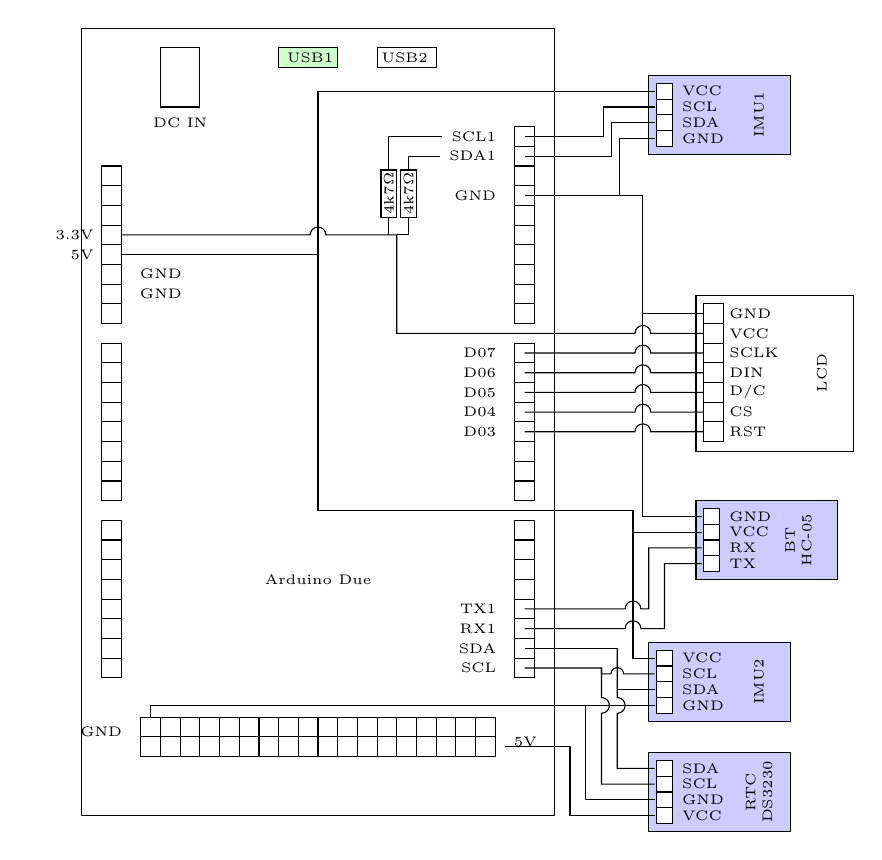
\begin{tikzpicture}
		\draw  (-3,5) rectangle (3,-5); % board
		\draw  (-2,4.75) rectangle (-1.5,4); % DC in
		\node [font=\tiny]   at(-1.75, 3.8){DC IN};
		\draw[fill=green!20]  (-0.5,4.75) rectangle (0.25,4.5); % USB 1
		\node [font=\tiny]   at(-0.1, 4.62){USB1};
		\draw  (0.75,4.75) rectangle (1.5,4.5); % USB 2
		\node [font=\tiny]   at(1.1, 4.62){USB2};
		\draw (2.5,3.75) rectangle (2.75,1.25);%SCL1
		\draw (2.5,3.5) -- (2.75, 3.5);%SDA1
		\draw (2.5,3.25) -- (2.75, 3.25);%AREF
		\draw (2.5,3) -- (2.75, 3);%GND
		\draw (2.5,2.75) -- (2.75, 2.75);%D13
		\draw (2.5,2.5) -- (2.75, 2.5);%D12
		\draw (2.5,2.25) -- (2.75, 2.25);%D11
		\draw (2.5,2) -- (2.75, 2);%D10
		\draw (2.5,1.75) -- (2.75, 1.75);%D09
		\draw (2.5,1.5) -- (2.75, 1.5);%D08
		\draw  (2.5,1) rectangle (2.75,-1);%D07
		\draw (2.5,0.75) -- (2.75, 0.75);%D06
		\draw (2.5,0.5) -- (2.75, 0.5);%D05
		\draw (2.5,0.25) -- (2.75, 0.25);%D04
		\draw (2.5,0) -- (2.75, 0);%D03
		\draw (2.5,-0.25) -- (2.75, -0.25);%D02
		\draw (2.5,-0.5) -- (2.75, -0.5); %TX0 -> 1
		\draw (2.5,-0.75) -- (2.75, -0.75); %RX0 -> 2
		\draw  (2.5,-1.25) rectangle (2.75,-3.25); %TX3
		\draw (2.5,-1.5) -- (2.75, -1.5); %RX3
		\draw (2.5,-1.75) -- (2.75, -1.75); %TX2
		\draw (2.5,-2) -- (2.75, -2); %RX2
		\draw (2.5,-2.25) -- (2.75, -2.25); %TX1
		\draw (2.5,-2.5) -- (2.75, -2.5); %RX1
		\draw (2.5,-2.75) -- (2.75, -2.75); %SDA
		\draw (2.5,-3) -- (2.75, -3); %SCL
		\draw  (-2.75,3.25) rectangle (-2.5,1.25);
		\draw (-2.75,3) -- (-2.5, 3);%IOREF
		\draw (-2.75,2.75) -- (-2.5, 2.75);%RESET
		\draw (-2.75,2.5) -- (-2.5, 2.5);%3.3V
		\draw (-2.75,2.25) -- (-2.5, 2.25);%5V
		\draw (-2.75,2) -- (-2.5, 2);%GND
		\draw (-2.75,1.75) -- (-2.5, 1.75);%GND
		\draw (-2.75,1.5) -- (-2.5, 1.5);%VIN
		\draw  (-2.75,1) rectangle (-2.5,-1); %A0
		\draw (-2.75,0.75) -- (-2.5, 0.75);%A1
		\draw (-2.75,0.5) -- (-2.5, 0.5);%A2
		\draw (-2.75,0.25) -- (-2.5, 0.25);%A3
		\draw (-2.75,0) -- (-2.5, 0);%A4
		\draw (-2.75,-0.25) -- (-2.5, -0.25);%A5
		\draw (-2.75,-0.5) -- (-2.5, -0.5); %A6
		\draw (-2.75,-0.75) -- (-2.5, -0.75); %A7
		\draw  (-2.75,-1.25) rectangle (-2.5,-3.25);%A08
		\draw (-2.75,-1.5) -- (-2.5, -1.5); %TX0 -> 1
		\draw (-2.75,-1.75) -- (-2.5, -1.75); %RX0 -> 2
		\draw (-2.75,-2) -- (-2.5, -2);%A4
		\draw (-2.75,-2.25) -- (-2.5, -2.25);%A5
		\draw (-2.75,-2.5) -- (-2.5, -2.5); %A6
		\draw (-2.75,-2.75) -- (-2.5, -2.75); %A7
		\draw (-2.75,-3) -- (-2.5, -3);%A4
		\draw  (-2.25,-3.75) rectangle (2.25,-4.25);
		\draw  (-2.25,-4) -- (2.25,-4);
		\draw  (-2,-3.75) -- (-2,-4.25);
		\draw  (-1.75,-3.75) -- (-1.75,-4.25);
		\draw  (-1.5,-3.75) -- (-1.5,-4.25);
		\draw  (-1.25,-3.75) -- (-1.25,-4.25);
		\draw  (-1,-3.75) -- (-1,-4.25);
		\draw  (-0.75,-3.75) -- (-0.75,-4.25);
		\draw  (-0.5,-3.75) -- (-0.5,-4.25);
		\draw  (-0.25,-3.75) -- (-0.25,-4.25);
		\draw  (0,-3.75) -- (0,-4.25);
		\draw  (0.25,-3.75) -- (0.25,-4.25);
		\draw  (0.5,-3.75) -- (0.5,-4.25);
		\draw  (0.75,-3.75) -- (0.75,-4.25);
		\draw  (1,-3.75) -- (1,-4.25);
		\draw  (1.25,-3.75) -- (1.25,-4.25);
		\draw  (1.5,-3.75) -- (1.5,-4.25);
		\draw  (1.75,-3.75) -- (1.75,-4.25);
		\draw  (2,-3.75) -- (2,-4.25);
		%IMU1
		\draw  [fill=blue!20](4.2,4.4) rectangle (6,3.4);
		\draw  [fill=white](4.3,4.3) rectangle (4.5,3.5);
		\draw  (4.3,4.1) -- (4.5,4.1);
		\draw  (4.3,3.9) -- (4.5,3.9);
		\draw  (4.3,3.7) -- (4.5,3.7);
		%IMU2
		\draw  [fill=blue!20](4.2,-2.8) rectangle (6,-3.8);
		\draw  [fill=white](4.3,-2.9) rectangle (4.5,-3.7);
		\draw  (4.3,-3.1) -- (4.5,-3.1);
		\draw  (4.3,-3.3) -- (4.5,-3.3);
		\draw  (4.3,-3.5) -- (4.5,-3.5);
		%BT
		\draw  [fill=blue!20](4.8,-1) rectangle (6.6,-2);
		\draw  [fill=white](4.9,-1.1) rectangle (5.1,-1.9);
		\draw  (4.9,-1.3) -- (5.1,-1.3);
		\draw  (4.9,-1.5) -- (5.1,-1.5);
		\draw  (4.9,-1.7) -- (5.1,-1.7);
		%RTC
		\draw  [fill=blue!20](4.2,-4.2) rectangle (6,-5.2);
		\draw  [fill=white](4.3,-4.3) rectangle (4.5,-5.1);
		\draw  (4.3,-4.5) -- (4.5,-4.5);
		\draw  (4.3,-4.7) -- (4.5,-4.7);
		\draw  (4.3,-4.9) -- (4.5,-4.9);
		%LCD
		\draw  (4.8,1.6) rectangle (6.8,-0.375);
		\draw  (4.9,1.5) rectangle (5.15,-0.25);
		\draw (4.9,1.25) -- (5.15, 1.25); 
		\draw (4.9,1) -- (5.15, 1); 
		\draw (4.9,0.75) -- (5.15, 0.75);
		\draw (4.9,0.5) -- (5.15, 0.5);
		\draw (4.9,0.25) -- (5.15, 0.25);
		\draw (4.9,0) -- (5.15, 0);
		\node[left, font=\tiny] (SCL1) at (2.625,3.625) {SCL1$\quad$};
		\node[left, font=\tiny] (SDA1) at (2.625,3.375) {SDA1$\quad$};
		\node[left, font=\tiny] (GND) at (2.625,2.875) {GND$\quad$};
		\node[left, font=\tiny] (D07) at (2.625,0.875) {D07$\quad$};
		\node[left, font=\tiny]  (D06) at (2.625,0.625) {D06$\quad$};
		\node[left, font=\tiny]  (D05) at (2.625,0.375) {D05$\quad$};
		\node[left, font=\tiny]  (D04) at (2.625,0.125) {D04$\quad$};
		\node[left, font=\tiny]  (D03) at (2.625,-0.125) {D03$\quad$};
		\node[left, font=\tiny]  (TX1) at (2.625,-2.375) {TX1$\quad$};
		\node[left, font=\tiny]  (RX1) at (2.625,-2.625) {RX1$\quad$};
		\node[left, font=\tiny]  (SDA) at (2.625,-2.875) {SDA$\quad$};
		\node[left, font=\tiny]  (SCL) at (2.625,-3.125) {SCL$\quad$};
		\node (GND3) at (-2.125,-3.875) {};
		\node[above left, font=\tiny] (GND4) at (-2.125,-4.125) {GND$\quad$};
		\node[below right, font=\tiny] (50V3) at (2.125,-3.875) {$\quad$5V};
		\node[right, font=\tiny] (50V4) at (2.125,-4.125) {};
		\node (33V)at (-2.625,2.375) {};
		\node[left, font=\tiny] at (-2.725,2.375) {$\quad$3.3V};
		\node (50V) at (-2.625,2.125) {};
		\node[left, font=\tiny]  at (-2.725,2.125) {$\quad$5V};
		\node[right, font=\tiny]  (GND1) at (-2.625,1.875) {$\quad$GND};
		\node[right, font=\tiny]  (GND2) at (-2.625,1.625) {$\quad$GND};
		\node(IMU1VCC) at (4.4,4.2) {};
		\node(IMU1SCL) at (4.4,4.0) {};
		\node(IMU1SDA) at (4.4,3.8) {};
		\node(IMU1GND) at (4.4,3.6) {};
		\node[right, font=\tiny] at (4.5,4.2) {VCC};
		\node[right, font=\tiny] at (4.5,4) {SCL};
		\node[right, font=\tiny] at (4.5,3.8) {SDA};
		\node[right, font=\tiny] at (4.5,3.6) {GND};
		\node[rotate=90, font=\tiny] at (5.6,3.9) {IMU1};
		\node(IMU2VCC) at (4.4,-3) {};
		\node(IMU2SCL) at (4.4,-3.2) {};
		\node(IMU2SDA) at (4.4,-3.4) {};
		\node(IMU2GND) at (4.4,-3.6) {};
		\node[right, font=\tiny] at (4.5,-3) {VCC};
		\node[right, font=\tiny] at (4.5,-3.2) {SCL};
		\node[right, font=\tiny] at (4.5,-3.4) {SDA};
		\node[right, font=\tiny] at (4.5,-3.6) {GND};
		\node[rotate=90, font=\tiny] at (5.6,-3.3) {IMU2};
		\node(BTGND) at (5,-1.2) {};
		\node(BTVCC) at (5,-1.4) {};
		\node(BTRX) at (5,-1.6) {};
		\node(BTTX) at (5,-1.8) {};
		\node[right, font=\tiny] at (5.1,-1.2) {GND};
		\node[right, font=\tiny] at (5.1,-1.4) {VCC};
		\node[right, font=\tiny] at (5.1,-1.6) {RX};
		\node[right, font=\tiny] at (5.1,-1.8) {TX};
		\node[rotate=90, font=\tiny, align=center] at (6.1,-1.5) {BT \\ HC-05};
		\node(RTCSDA) at (4.4,-4.4) {};
		\node(RTCSCL) at (4.4,-4.6) {};
		\node(RTCGND) at (4.4,-4.8) {};
		\node(RTCVCC) at (4.4,-5) {};
		\node[right, font=\tiny] at (4.5,-4.4) {SDA};
		\node[right, font=\tiny] at (4.5,-4.6) {SCL};
		\node[right, font=\tiny] at (4.5,-4.8) {GND};
		\node[right, font=\tiny] at (4.5,-5) {VCC};
		\node[rotate=90, font=\tiny, align=center] at (5.6,-4.7) {RTC \\ DS3230};
		\node (LCDGND) at (5.025,1.375) {};
		\node (LCDVCC) at (5.025,1.125) {};
		\node (LCDD07) at (5.025,0.875) {};
		\node (LCDD06) at (5.025,0.625) {};
		\node (LCDD05) at (5.025,0.375) {};
		\node (LCDD04) at (5.025,0.125) {};
		\node (LCDD03) at (5.025,-0.125) {};
		\node[right, font=\tiny] at (5.1,1.375) {GND};
		\node[right, font=\tiny] at (5.1,1.125) {VCC};
		\node[right, font=\tiny] at (5.1,0.875) {SCLK};
		\node[right, font=\tiny] at (5.1,0.625) {DIN};
		\node[right, font=\tiny] at (5.1,0.375) {D/C};
		\node[right, font=\tiny] at (5.1,0.125) {CS};
		\node[right, font=\tiny] at (5.1,-0.125) {RST};
		\node[rotate=90, font=\tiny, align=center] at (6.4,0.625) {LCD};
		\draw(SCL1) --(3.625,3.625) |- (IMU1SCL);
		\draw  (SDA1)--(3.725,3.375)  |-(IMU1SDA);
		\draw  (GND) -- (3.825,2.875)|- (IMU1GND);
		\draw  (50V) --(0,2.125) |- (IMU1VCC);
		\draw  (50V) --(0,2.125)--(0,-1.125)--(4,-1.125) |- (IMU2VCC);
		\draw (SDA) -- (3.8,-2.875) |-(IMU2SDA);
		\draw(SCL) -- (3.6,-3.125) |- (3.72,-3.2) arc(180:0:0.08)--(IMU2SCL);4.4,-3.2
		\draw (GND3) |- (IMU2GND);
		\draw(4,-1.125) |- (BTVCC);
		\draw(TX1) --(3.9,-2.375) arc(180:0:0.1)--(4.2,-2.375) |-(BTRX);
		\draw(RX1) --(3.9,-2.625) arc(180:0:0.1)--(4.4,-2.625) |-(BTTX);
		\draw  (GND) -- (4.125,2.875)|- (BTGND);
		\draw  (4.125,1.375) -- (LCDGND);
		\draw (33V) -- (-0.1,2.375) arc(180:0:0.1)-- (1,2.375) |-(4.025,1.125) arc(180:0:0.1)-- (LCDVCC);
		\draw (D07) --(4.025,0.875) arc(180:0:0.1)-- (LCDD07);
		\draw (D06) --(4.025,0.625) arc(180:0:0.1)-- (LCDD06);
		\draw (D05) --(4.025,0.375) arc(180:0:0.1)--(LCDD05);
		\draw (D04) --(4.025,0.125) arc(180:0:0.1)-- (LCDD04);
		\draw (D03) --(4.025,-0.125) arc(180:0:0.1)-- (LCDD03);
		\draw(3.8,-2.875) --(3.8,-3.5) arc(90:-90:0.1)|-(RTCSDA);
		\draw(3.6,-3.125)--(3.6,-3.5) arc(90:-90:0.1) |-(RTCSCL);
		\draw(3.4,-3.6) |-(RTCGND);
		\draw(50V4) -- (3.2, -4.125) |- (RTCVCC);
		\draw(0.9,2.375)--(0.9,2.6);
		\draw(1,2.375)-|(1.15,2.6);
		\draw(0.9,3.2)|-(SCL1);
		\draw(1.15,3.2) |-(SDA1);
		\draw  (1.05,3.2) rectangle (1.25,2.6);
		\draw  (0.8,3.2) rectangle (1.,2.6);
		\node[font=\tiny, rotate=90] at (0.9,2.9) {4k7$\Omega$};
		\node[font=\tiny, rotate=90] at (1.15,2.9) {4k7$\Omega$};
		\node[font=\tiny] at (0,-2) {Arduino Due};
	\end{tikzpicture}
	\caption{Schemat budowy urządzenia pomiarowego opartego o~komputer Arduino.}
													
	\label{fig:device:circuitDiagram}
\end{figure}